\documentclass[11pt]{article}

\usepackage{fullpage}
\usepackage[margin=1in]{geometry}
\usepackage{graphicx}
\usepackage{amsmath,amsthm,amssymb}
\usepackage{hyperref}
\usepackage{biblatex}
\usepackage[dvipsnames]{xcolor}



\addbibresource{references.bib}

\graphicspath{ {./} }

% --------------------------------------------------------------
%                         Start here
% --------------------------------------------------------------

\begin{document}

\title{C Group Project Final Report}
\author{Hoang Vu, Kaiyan Fan, Xuan(Tom) Zhao, Zelin(Daniel) Deng}

\maketitle

\noindent In this group project, we have accomplished ARM11-based emulator and assembler, as well as Tetris\texttt{++} as our extension. Below is our final report.

% --------------------------------------------------------------
%                         ARM11 Assembler
% --------------------------------------------------------------

\section{ARM11 Assembler}

% --------------------------------------------
%             Assembler Structure
% --------------------------------------------
\subsection{Assembly Structure}
\begin{figure}[!ht]
  \centering
  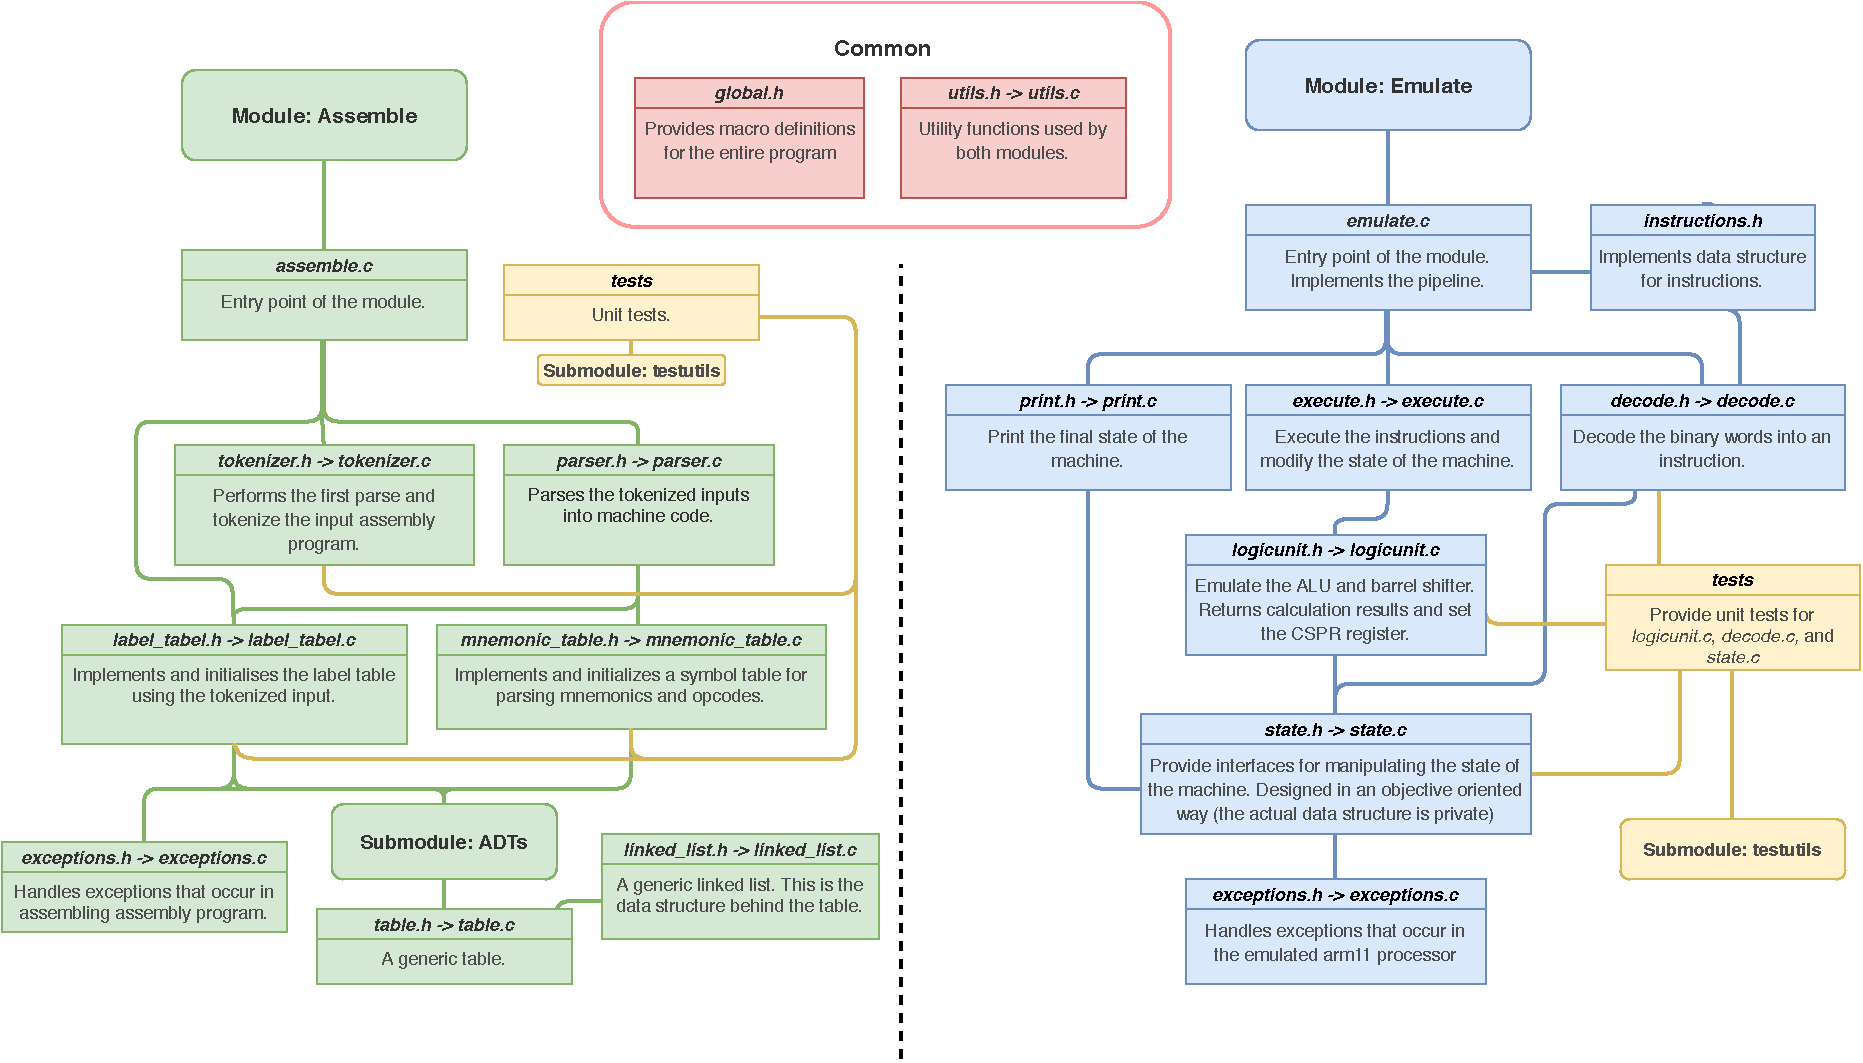
\includegraphics[scale = 0.5]{project_structure_final.pdf}
  \caption{An UML Diagram of the Overall ARM11 Project Structure}
  \label{part1:UML}
\end{figure}
\begin{flushleft}
The functions of different parts are described in the diagram above. For the assembler, there are three main parts: symbol table, tokenizer, and parser. We have created an abstract data structure \texttt{linked\_list} to construct a genetic table for both the \texttt{label\_table} and \texttt{mnemonic\_table}. First, the assembly code is tokenized into an \texttt{assembly\_line}(a \texttt{struct} containing label, opcode, and operand fields) by \texttt{tokenizer}; then, it will be parsed into binary code by \texttt{parser}. We have previously implemented another structure using the structure we defined in \texttt{instructions.h} in our emulator, but our current version is simpler and more elegant.
\end{flushleft}

% --------------------------------------------
%             Implementation
% --------------------------------------------

\subsection{Implementation}
\begin{flushleft}
We have utilized several \texttt{struct} in our assembler:
\begin{itemize}
\item \texttt{symbol\_table\_t} is the mapping between label and their address, implemented as a linked-list.
\item \texttt{assembly\_line} contains \texttt{label}, \texttt{opcode}, an array of \texttt{operands} strings for each operand fields, and a \texttt{location\_counter} for tracking the address of a label in instruction memory.
\item \texttt{assembly\_program} is made up by an array of \texttt{assembly\_line}s.
\item \texttt{mnemonic\_t} contains the instruction type and a pre-set 32-bit binary according to opcode and other clues.
\item \texttt{machine\_code} contains the binary code of an entire assembly file and the line count of binary code.
\end{itemize}
One line of assembly code will first be tokenized into \texttt{assembly\_line} with the \texttt{location\_counter} increases for each line of assembly. Meanwhile, if a label is encountered, the \texttt{location\_counter} will be the address of the label and will be inserted into the \texttt{label\_table}. Next, a new \texttt{mnemonic\_t} structure, where the pre-set binary and instruction type are stored, will be generated according to the opcode field of the \texttt{assembly\_line}. Finally, the \texttt{parser} will break down different operand fields, set the rest of the bits according to the pattern of operands(e.g. hash expression), and then append the binary to the \texttt{machine\_code}. After parsing, the \texttt{machine\_code} will contain the binary encoding, which will be written by the \texttt{write\_binary\_file} function in \texttt{utils.c}.
\end{flushleft}
\begin{flushleft}
Additionally, we have added the ability to handle possible exceptions and encapsulated as many structures as possible. For instance, we have written getters and setters in out table implementation, and replaced \texttt{malloc} with checking with \texttt{eMalloc} in \texttt{utils.c}, and for \texttt{calloc} and \texttt{realloc} as well.
\end{flushleft}


% --------------------------------------------------------------
%                         Extension: Tetris++
% --------------------------------------------------------------

\section{Extension: Tetris\texttt{++}}

\begin{figure}[!ht]
  \centering
  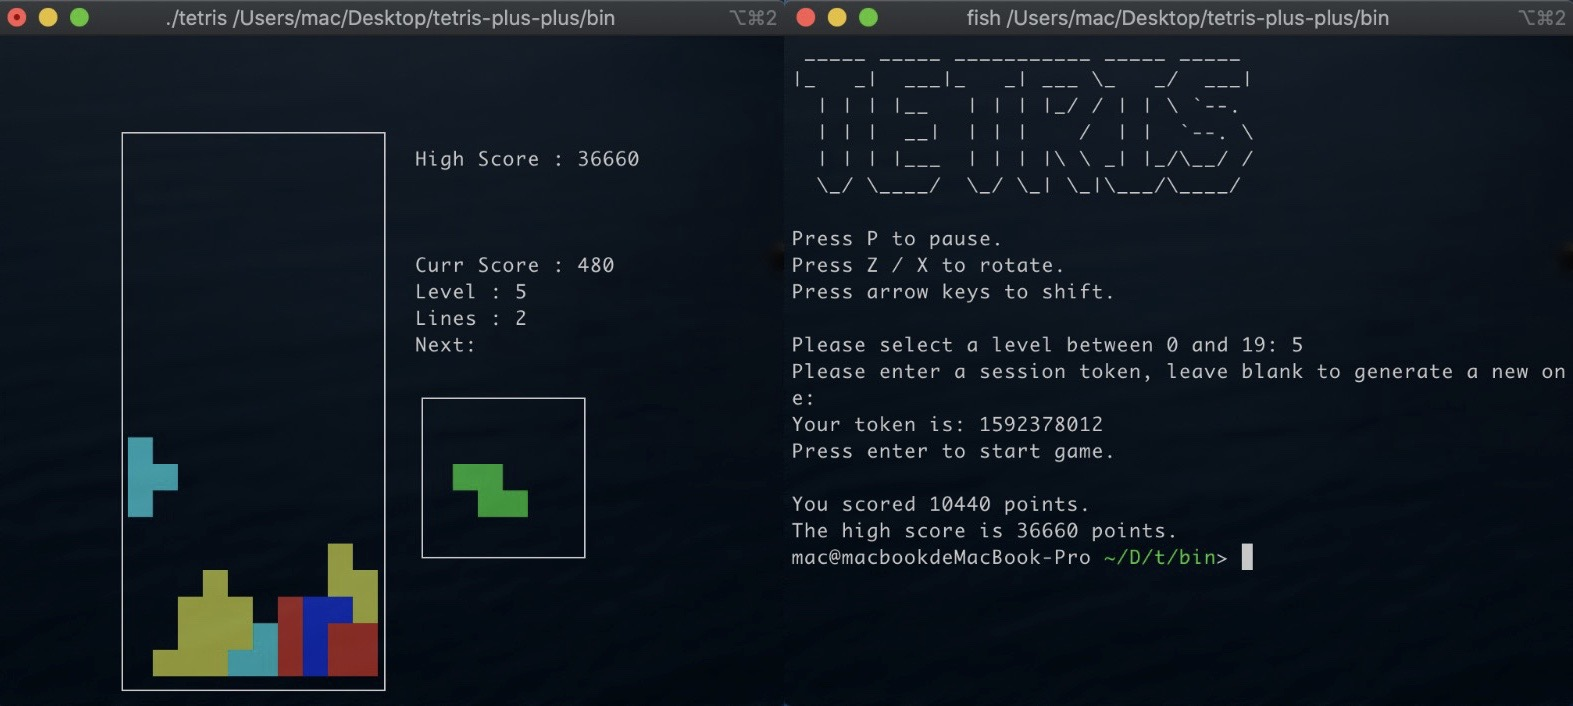
\includegraphics[scale = 0.25]{tetris.jpg}
    \caption{A Demo of the Tetris Interface in Command Line}
  \label{part2:jpg}
\end{figure}


% --------------------------------------------
%             Description
% --------------------------------------------

\subsection{Description}

\begin{flushleft}
Our extension is the classic Tetris game, but with the ability to play with console or accelerometer on Raspberry Pi against human or AI. It's a game loved by all of our team members, as well as a way to stay healthy both mentally and physically during the quarantine caused by the COVID-19 global pandemic. It is built upon ncurses for the command line version, and has a Raspberry Pi version as well. We have implemented AI in two different ways: one uses genetic algorithm and the other uses reinforcement learning.
\end{flushleft}

% --------------------------------------------
%             How to play
% --------------------------------------------

\subsection{How to Play}

\begin{flushleft}
To play it on terminal, run \texttt{make core} in the root directory \texttt{\textbackslash tetris-plus-plus} and go to \texttt{\textbackslash bin} to run \texttt{./tetris}. The player has to pick a level to start with, then chooses to put in a random number as a seed. The higher the level, the faster the game. The control keys are shown on the welcome screen: press \texttt{P} to pause, press \texttt{Z / X} to rotate block, press arrow keys to move left or right.
\end{flushleft}

\begin{flushleft}
To train the AI implemented by genetic algorithm, run \texttt{make genetic-ai} in the root directory \texttt{\textbackslash tetris-plus-plus} and go to \texttt{\textbackslash bin} to run \texttt{./train}. The training progress will be displayed in the command line. After the training of each generation of parameters, the result will be written to a text file named \texttt{training\_progress.txt} in \texttt{\textbackslash bin}. You can continue training from the text file by running \texttt{./train training\_progress.txt}.
\end{flushleft}

\begin{flushleft}
To watch the genetic AI play, run \texttt{make genetic-ai} in the root directory \texttt{\textbackslash tetris-plus-plus} and go to \texttt{\textbackslash bin} to run \texttt{./genetic-ai-play}.
\end{flushleft}

\begin{flushleft}
To train the AI implemented by reinforcement learning, run \texttt{make rl-train} in the root directory to generate the executable and \texttt{./bin/rltrain} to watch as it trains.
\end{flushleft}

\begin{flushleft}
To play it on Raspberry pi using console/accelerometer, run 
\end{flushleft}

\begin{flushleft}
On Raspberry Pi, you can play it with ...
\end{flushleft}

% --------------------------------------------
%        Challenges and Problems
% --------------------------------------------

\subsection{Challenges and Problems}

\subsubsection{Game Engine}
\begin{flushleft}
The core algorithm of Tetris is relatively simple, to help with consistency and standardisation, we chose to use the reverse engineering of the 1989 NES Tetris as the standard for how the game should behave \cite{tetrisreverseengineering}. We chose this version as it is a popular implementation that all future versions evolved from. The challenge is to design a system of inputs and outputs that are versatile enough for all of our extensions, whilst being easy to use for the users. For example, games employ a system called DAS (delayed auto shift), to make sure both "taps" and "holds" of a key are being registered correctly, and getting the timing right for this part was challenging. In the end we decided to sample the input at the rate of 60 times per second, which allowed seamless user input without the use of multi-threading. 
\end{flushleft}

\subsubsection{Raspberry Pi}
\colorbox{yellow}{(Kaiyan could elaborate more on this)}
\begin{flushleft}
Write here...
\end{flushleft}

\subsubsection{Tetris AI}
To make the most out of our game engine and to make the game more interesting, we have decided to build Tetris Bots to compete with users. Here, we have taken this opportunity to experiment two famous algorithms, Genetic Algorithm which is mainly used in optimisation problems, and Reinforcement Learning, specifically using the Q-Learning Model. The biggest common challenge for both AI implementations, is the evaluation of a \textit{good} move. The instinct tells us that a good move should fit the shape of the bottom layer which will make the line as flat as possible, but it is hard to quantify this. After spending a few hours on research, we have decided to use a modified policy taken from \cite{tetrisai} including \textit{aggregate height, number of lines cleared, number of holes and bumpiness}, as illustrated.  

\paragraph{Tetris AI - Genetic Algorithm}
\begin{flushleft}
The challenge of the genetic AI is not its implementation, but its design and also to represent a good move. One issue is how to design a good way to reduce calculations and changes to arrays in order to save time during training. For instance, our implementation has separated the current generation and its children into two arrays instead of merging them together. We have also encapsulated the clone functions for the state and the grid, though partial clone might be faster. It turns out that the training progress is comparatively fast if running on a multi-core server.
\end{flushleft}


\paragraph{Tetris AI - Reinforcement Learning}
\begin{flushleft}
The fundamental idea is to reward the bot when it performs a beneficial move and comparing that against its past experience. To do this, we need to give our agent a memory, or more precisely the state of the game along with the outcome of each action. On first sight, the Tetris Board can be represented as a binary matrix, where 0 for a blank and 1 for an occupied cell. However, this can easily add up to ${2^{300}}$ possible states, including the states of our block. Hashing was our first solution, which quickly shows it weakness as not only it was challenging coming up with a hash function that captures the state of the block and the board. Our second attempt was to encode the Tetris Board using an array of heights, relative to the height of the first column. From our research, this is usually solved by employing other AI techniques, mainly Deep Learning to find a good mapping for dimensionality reduction. However, due to time constraints of implementing such network, and a further constraint of training time, we leave this as a future improvement.
\end{flushleft}

    
% --------------------------------------------
%             Testing
% --------------------------------------------

\subsection{Testing}
\begin{flushleft}
We have implemented test cases for each individual module in our extension the same way we had done in emulator and assembler. We have unit tests for every function that can be tested in the core module. Integration tests in this module is done by trying edge cases in the input fields, and by spending time manually running the program. More than 20 hours test time has been spent on the core module alone. 
\end{flushleft}

\begin{flushleft}
Due to the limited amount of time for our extension, only basic testings have been carried out for the core functionalities of our game. This includes game logic in the  engine, 
For genetic algorithm, the test cases only cover some functions. To validate whether the training is on the right track, we run it on a server for a while to see if the number of lines cleared is increasing after training each generation. For reinforcement learning...
\end{flushleft}

\begin{flushleft}
\colorbox{yellow}{(Discuss about the effectiveness of the testing...Daniel and Kaiyan could say more here)}
\end{flushleft}

% --------------------------------------------------------------
%                         Reflection
% --------------------------------------------------------------

\section{Reflection}

% --------------------------------------------
%             Group reflection
% --------------------------------------------

\subsection{Group reflection}
\begin{flushleft}
Our group holds a high standard during our development. With our frequent use of git, we have communicated efficiently, divided work by using git issues, and reviewed each other's codes using merge requests. We used git issues to create a separate branch for every new development, which is merged into development when it passes our own unit tests; development is then merged into master when it passes all the provided test cases. Each group member has also contributed in writing test cases for different modules. This work flow helps us avoid bad merge conflicts or potential bugs. 
\end{flushleft}

\begin{flushleft}
Because of our clear communication and agile workflow, the difference in timezone worked in our favour as it allowed a near 24 hour development cycle with enough overlap for code review sessions. 
\end{flushleft}

\begin{flushleft}
There remains potential for improvement as well. Before designing the assembler, we should have done research about the function of assembler, as well as common design structures used. We could have also managed our time better; for example deciding on what to do for the extension earlier so we have more time for improvements. 
\end{flushleft}

% --------------------------------------------
%             Individual Reflection
% --------------------------------------------

\subsection{Individual Reflection}
\begin{itemize}
    \item Hoang Vu: I truly see the power of teamwork after this group project. As a team, we have clearly shown the effectiveness of group discussions and the importance of feedback. As individuals, we have all shown a high level of dedication to our work, as well as review each other's work. Having our own strengths, our ideas were very creative and diverse, which ultimately led to the success of this project.  Personally, my biggest lesson was being able to write reusable codes which I got from writing our \texttt{ADT hash\_table}. This was then used in \texttt{mnemonic\_table, label\_table} and \texttt{q\_table}. One possible improvement is that we should be discussing ideas on how to approach problems together before coding it up, this will reduce the amount of time that we waste from completely re-designing a particular functionality after a negative feedback.    
    \item Kaiyan Fan:
    \item Xuan(Tom) Zhao: During this group project, I have developed the decoder in emulator and part of the parser in assembler. I wrote the AI with genetic algorithm in our extension and trained different version of it. At first, I thought communication is my limiting factor, but it turns out that both the code reviews and our zoom meetings are rather productive. The real limiting factor that I need to tackle is to add more care when writing code. The most important lesson I have learned from this group work is that design is the most pivotal step, and a good design could reduce code size and complexity, and eventually less bugs to deal with.
    \item Zelin(Daniel) Deng: Whilst Kaiyan did a brilliant job structuring the C dependencies, I was in charge of the physical layout. On top of writing my share of the C code, I structured the repositories and Makefiles for versatility and modularity. The rest of the group did a great job complimenting my strength in keeping files organised, and weaknesses in writing unit tests. I hope I complimented theirs as well. For future group work, I would spend more time helping to write tests for my teammates, in addition to testing my own code.  
\end{itemize}


\printbibliography

\end{document}